\chapter{Аналитический раздел}

Одной из главных причин низкой скорости обработки запросов является работа с базой данных (БД), которая не оптимизирована: нерациональные запросы, некорректное использование индексов, неоптимальные значения параметров конфигурации. 

Оптимизация производительности сводится к следующим задачам: 
\begin{enumerate}
    \item корректировка параметров СУБД;
    \item денормализация данных;
    \item выявление медленных запросов и их анализ:
        \begin{enumerate}
            \item корректировка запросов;
            \item создание индексов.
        \end{enumerate}
\end{enumerate}

Основным приемом увеличения производительности выполнения запросов к базе данных является индексирование. Индексы представляют собой структуры, которые помогают MySQL эффективно извлекать данные. Они критичны для достижения хорошей производительности, но многие часто забывают о них или плохо понимают их смысл, поэтому индексирование является главной причиной проблем с производительностью в реальных условиях. \cite{zaitsev}

В основном индексы находятся в памяти и поэтому увеличивают производительность путем оптимизации обращений к дисковой памяти.

Индексы следует создавать по мере обнаружения медленных запросов. В этом поможет \textit{slow log} в MySQL. Запросы, которые выполняются более 1 секунды, являются первыми кандидатами на оптимизацию. \cite{ruhighload-mysql-indexes} Конечно, говорить о том, сколько секунд считать медленным запросом зависит от конкретной задачи. В основном такие запросы используют JOIN оператор для соединения двух и более таблиц.

СУБД решают задачу выбора индекса для выполнения конкретного sql запроса на БД, заполненной реальными данными. Чтобы понять, какой индекс необходимо построить для оптимизации выполнения sql запроса администратору БД необходимо учитывать:
\begin{enumerate}
    \item реальные данные, которыми заполнена БД
    \item статистику запросов;
    \item правила работы СУБД с индексами;
    \item правила работы СУБД при соединении таблиц (для сложных запросов).
\end{enumerate}

Если абстрагироваться от реальных данных и статистики запросов, то зная правила работы СУБД можно сделать предположения, какие индексы могла бы использовать СУБД. 

В данной работе предлагаются алгоритмы, которые по заданному sql запросу вернут список индексов, которые могли бы использоваться СУБД при выполнении этого запроса. Предложенные алгоритмы облегачат работу администраторов БД, которым останется только принять решение, какой именно индекс построить из предложенного списка возможных индексов.

\section{Структура индексов в MySQL InnoDB}

Индексы представляют собой структуры, которые помогают эффективно извлекать данные.
В СУБД MySQL InnoDB используются Btree индексы, основанные на структуре данных B+tree Рисунок \ref{img:btree-structure}.

\begin{figure}[H]
  \centering
  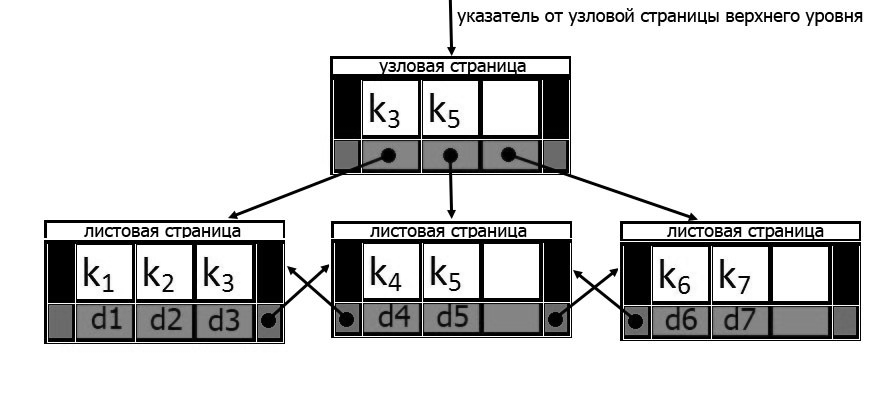
\includegraphics[scale=0.5]{btree.png}
  \caption{Структура данных B+tree.}
  \label{img:btree-structure}
\end{figure}

Где
$k_i$ - ключи ($k_i < k_i + 1$),
$d_i$ - данные.

Сложность поиска в линейной структуре данных $O(N)$, а в B+tree - $log(K)+N_k$, где $k$ — количество уровней, а $N_k$ — количество элементов в узле. Поэтому индексы, использующие структуру данных B+tree, эффективны для поиска данных. Для оптимизации поиска по диапазону в листовых страницах есть указатели на следующую и предыдущую листовую страницу.

Далее в качестве примера будет рассматриваться таблица $poet (poet\_id, last\_name, first\_name, dob, country)$

\begin{table}[h]
\caption{Таблица поэтов}
\medskip
\begin{tabular}{|l|l|l|l|l|}
\hline
poet\_id & last\_name & first\_name & dob & country\\
\hline
1 & “Блок“ & “Александр“ & 1880 & “ru”\\
2 & “Фет“ & “Афанасий“ & 1820 & “ru”\\
3 & “Лермонтов“ & “Михаил“ & 1814 & “ru”\\
4 & “Ильф“ & “Илья“ & 1897 & “ru”\\
5 & “Пушкин“ & “Александр“ & 1799 & “ru”\\
6 & “Булгаков“ & “Михаил“ & 1891 & “ru”\\
7 & “Есенин“ & “Сергей“ & 1895 & “ru”\\
\hline
\end{tabular}
\end{table}

\subsection{Кластерный индекс}

В InnoDB данные хранятся в структуре B+tree, где в узловых страницах хранятся первичные ключи, а в листовых страницах хранятся данные. Такое дерево называется кластерным индексом. Над таблицей можно построить только один кластерный индекс, поскольку невозможно хранить одну и ту же запись одновременно в двух местах. Однако часть или всю запись можно хранить в нескольких местах, что будет использоваться в покрывающих индексах \ref{section:covering-index}.

По рисуноку \ref{img:btree-structure}, где $k_1 \ldots k_7$ - первичные ключи ($poet\_id$), $k_i = i$; $d_1 \ldots d_7$ - данные.

$d_1$ = “Блок“, “Александр“, 1880, “ru”; 

$d_2$ = “Фет“, “Афанасий“, 1820, “ru”;

$\ldots$

Если вы не задаёте первичный ключ, то MySQL неявно добавит скрытое поле и кластерезует данные по нему, но доступа к нему не даст. Отсюда следует, что первичный ключ желательно явно создавать самим.

Характерной проблемой кластерного индекса является то, что при вставке в страницу, если в ней закончилось место, создается новая пустая страница. Из-за этого, со временем появляется много пустующего места и таблицы InnoDB начинают занимать много места. Данная проблема решается командой $OPTIMAZE\:TABLE\;table\_name;$

\subsection{Вторичный индекс}

Для оптимизации конкретных запросов используются вторичные индексы (далее просто индексы). В узловых страницах индексов хранятся поля, по которым создан этот индекс, а в листовых страницах хранится значение первичного ключа. Для каждой таблицы в одном запросе используется только один индекс. При использовании в запросах индекса, сначала будет найдено значение первичного ключа, затем по этому значению будут найдены данные в кластерном индексе. Поэтому при создании вторичного индекса, в конец неявно добавляется первичный ключ.

На рисунке \ref{img:index-structure} показан индекс по полю (dob). Где $k_1 \ldots k_7$ - ключи, по которым построен индекс; $k_1$ = “1799”, $k_2$ = “1814”, $k_3$ = “1820”, $\ldots$; $p_1 \ldots p_7$ - первичные ключи ($poet\_id$); $p_i = i$.

\begin{figure}[H]
  \centering
  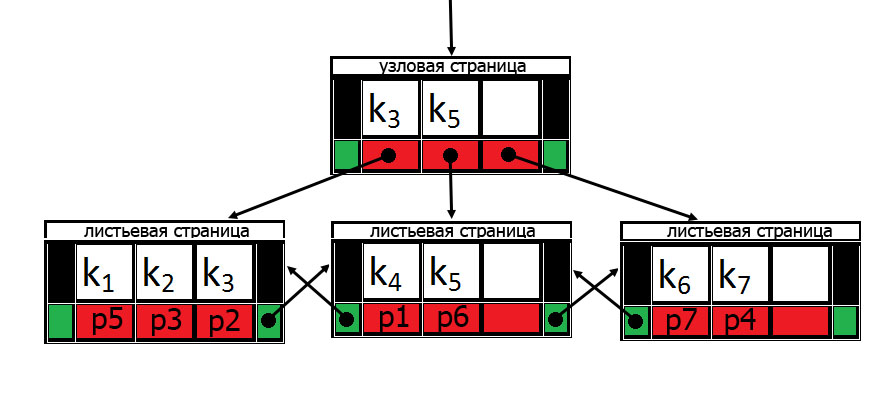
\includegraphics[scale=0.5]{index-structure.png}
  \caption{Структура вторичного индекса}
  \label{img:index-structure}
\end{figure}

\subsection{Составной индекс}

Чтобы правильно использовать составные индексы, необходимо понять структуру их хранения. Все работает точно так же, как и для обычного индекса, но для значений используются значения всех входящих колонок сразу, по которым строится индекс. Составной индекс может использоваться частично, но только по самому левому префиксу.

Если построить индекс по полям $(dob, last\_name)$, то для рисунка \ref{img:index-structure}
$k_1$ = “1799Пушкин”, $k_2$ = “1814Лермонтов”, $k_3$ = “1820Фет”, $\ldots$

Составной индекс может использоваться как \textbf{частичный индекс}, являющийся левым префиксом составного индекса. 

\subsection{Селективность индексов}

Чем меньше строк войдет в выборку, тем быстрее будет работать поиск по ней. Если рассматривать таблицы с равномерно распределенными значениями в полях, то условие $=$ более селективно, чем условия $>$, $<=$, $>=$, $<$.

\subsection{Покрывающий индекс}
\label{section:covering-index}

Индекс называется покрывающим, если в нем есть все поля, используемые в запросе. Покрывающие индексы позволяют имитировать кластерные индексы. Индексы, как правило, находятся в памяти, и не потребуется долгих операций ввода/вывода с диска. 

Для запроса на листинге \ref{sql:covering-index} строим индекс $(last\_name, dob)$.
\begin{lstlisting}[language=sql, label=sql:covering-index, caption={запрос для covering-index}]
SELECT last_name, dob
FROM poet
WHERE last_name = "Пушкин"
\end{lstlisting}


\section{Индексы для простых запросов}

Чтобы построить индексы для простых запросов (т.е. без соединения таблиц) необходимо воспользоваться простыми правилами.

\subsection{Индексы для WHERE}

Для запроса на листинге \ref{sql:index-on-where} можно построить индексы \textit{(dob, last\_name)} и \textit{(last_name, dob)}.
\begin{lstlisting}[language=sql, label=sql:index-on-where, caption={запрос для index-on-where}]
SELECT * 
FROM poet
WHERE last_name = ”Пушкин” 
    AND dob = 1799
\end{lstlisting}

Рассмотрим работу индексов на примере индекса \textit{(a, b, c)}, где \textit{a, b} - числа, \textit{c} - строка.

\paragraph{Примеры запросов, к которым применяется индекс \textit{(a, b, c)}}

\begin{enumerate}
\item \textit{a = 5 AND b = 10 AND c="Hello world"}
\item \textit{a = 5}
\item \textit{a > 5}  
\item \textit{a = 5 AND b = 10} 
\item \textit{a = 5 AND b = 10 AND c LIKE "Hello w\%"} 
\item \textit{a = 5 AND b IN (2,3)} (\textit{IN} - рассматривается как поиск по диапазону)
\end{enumerate}

\paragraph{Примеры запросов, к которым не применяется индекс \textit{(a, b, c)}}

\begin{enumerate}
\item \textit{b = 5}
\item \textit{a=5 AND b=10 AND c LIKE "\% world"}
\item \textit{a=5 AND c=10}
\item \textit{a>5 AND b=2}
\end{enumerate}



\subsection{Индексы при сортировке}

Чтобы получить отсортированную последовательность данных, MySQL достаточно будет пройтись по дереву, т.к. в индексе данные хранятся в отсортированном виде. 

Для запроса на листинге \ref{sql:index-order1} строим индекс $(dob)$.
\begin{lstlisting}[language=sql, label=sql:index-order1, caption={запрос для index-order}]
SELECT * 
FROM poet
ORDER BY dob
\end{lstlisting}

Для запроса на листинге \ref{sql:index-order2} строим индекс $(country, dob)$. В индексе находим строки, удовлетворяющие условию $country="ru"$, а в этой выборке строки уже отсортированы по $dob$.
\begin{lstlisting}[language=sql, label=sql:index-order2, caption={запрос для index-order}]
SELECT * 
FROM poet
WHERE country="ru" 
ORDER BY dob
\end{lstlisting}

Для запроса на листинге \ref{sql:index-order3} строим индекс $(dob)$. $GROUP\:BY$ возьмет уже отсортированные строки из индекса и уберет повторы, а т.к. строки уже отсортированные - $ORDER\:BY$ всего лишь задаст, в каком порядке выводить данные. 
\begin{lstlisting}[language=sql, label=sql:index-order3, caption={запрос для index-order}]
SELECT *
FROM poet
GROUP BY dob
ORDER BY dob
\end{lstlisting}


\paragraph{Index-order правила}

Рассмотрим работу индексов на примере индекса $(a, b)$, где $a, b$ - числа.

Примеры работы индекса $(a, b)$:
\begin{enumerate}
\item сортировка по первой колонке
\item первая колонка в условии $WHERE$, и сортировка по второй колонке
\item первая колонка в условии $WHERE$ и сортировка по первой колонке
\item сортировка по двум колонкам и обе в одну сторону
\end{enumerate}

Примеры, когда индекс $(a, b)$ не работает:
\begin{enumerate}
\item $ORDER\:BY \; b$ (т.к. $b$ - не левый префикс индекса)
\item $WHERE a>5 \; ORDER\,BY\:b$ \\
Пример данных в индексе $(a, b)$: $a=6,\:b=2; \; a=6,\:b=3; \; a=7,\: b=0; \; a=8,\:b=1$.\\
MySQL сделает выборку по условию $a>5$, но в этой выборке строки не отсортированы по $b$.
\item $WHERE a\:IN\:(1,2) \; ORDER\:BY\:b$ (тоже самое, что и в предыдущем запросе)
\item сортировка разных столбцов в разных направлениях (чтобы обойти это, можно сделать виртуальную колонку, например, перед числом поставить минус)
\end{enumerate}

\subsection{Агрегирующие функции MIN, MAX}

Так как данные в индексе отсортированы, то для нахождения минимального или максимального значения достаточно взять крайнее значение.

Для запроса на листинге \ref{sql:index-aggr1} строим индекс $(dob)$.
\begin{lstlisting}[language=sql, label=sql:index-aggr1, caption={запрос для index-aggr}]
SELECT MAX(dob) 
FROM poet;
\end{lstlisting}

Для запроса на листинге \ref{sql:index-aggr2} строим индекс $(first\_name, dob)$.
\begin{lstlisting}[language=sql, label=sql:index-aggr2, caption={запрос для index-aggr}]
SELECT MAX(dob) 
FROM poet
GROUP BY first_name
\end{lstlisting}



\section{Индексы для сложных запросов}

\subsection{Общие правила}
\begin{enumerate}
\item в одном запросе для каждой таблицы используется максимум один индекс;
\item в выражениях \textit{GROUP BY} и \textit{ORDER BY} поля только из одной таблицы.
\end{enumerate}
